% Options for packages loaded elsewhere
\PassOptionsToPackage{unicode}{hyperref}
\PassOptionsToPackage{hyphens}{url}
%
\documentclass[
]{article}
\usepackage{amsmath,amssymb}
\usepackage{iftex}
\ifPDFTeX
  \usepackage[T1]{fontenc}
  \usepackage[utf8]{inputenc}
  \usepackage{textcomp} % provide euro and other symbols
\else % if luatex or xetex
  \usepackage{unicode-math} % this also loads fontspec
  \defaultfontfeatures{Scale=MatchLowercase}
  \defaultfontfeatures[\rmfamily]{Ligatures=TeX,Scale=1}
\fi
\usepackage{lmodern}
\ifPDFTeX\else
  % xetex/luatex font selection
\fi
% Use upquote if available, for straight quotes in verbatim environments
\IfFileExists{upquote.sty}{\usepackage{upquote}}{}
\IfFileExists{microtype.sty}{% use microtype if available
  \usepackage[]{microtype}
  \UseMicrotypeSet[protrusion]{basicmath} % disable protrusion for tt fonts
}{}
\makeatletter
\@ifundefined{KOMAClassName}{% if non-KOMA class
  \IfFileExists{parskip.sty}{%
    \usepackage{parskip}
  }{% else
    \setlength{\parindent}{0pt}
    \setlength{\parskip}{6pt plus 2pt minus 1pt}}
}{% if KOMA class
  \KOMAoptions{parskip=half}}
\makeatother
\usepackage{xcolor}
\usepackage[margin=1in]{geometry}
\usepackage{color}
\usepackage{fancyvrb}
\newcommand{\VerbBar}{|}
\newcommand{\VERB}{\Verb[commandchars=\\\{\}]}
\DefineVerbatimEnvironment{Highlighting}{Verbatim}{commandchars=\\\{\}}
% Add ',fontsize=\small' for more characters per line
\usepackage{framed}
\definecolor{shadecolor}{RGB}{248,248,248}
\newenvironment{Shaded}{\begin{snugshade}}{\end{snugshade}}
\newcommand{\AlertTok}[1]{\textcolor[rgb]{0.94,0.16,0.16}{#1}}
\newcommand{\AnnotationTok}[1]{\textcolor[rgb]{0.56,0.35,0.01}{\textbf{\textit{#1}}}}
\newcommand{\AttributeTok}[1]{\textcolor[rgb]{0.13,0.29,0.53}{#1}}
\newcommand{\BaseNTok}[1]{\textcolor[rgb]{0.00,0.00,0.81}{#1}}
\newcommand{\BuiltInTok}[1]{#1}
\newcommand{\CharTok}[1]{\textcolor[rgb]{0.31,0.60,0.02}{#1}}
\newcommand{\CommentTok}[1]{\textcolor[rgb]{0.56,0.35,0.01}{\textit{#1}}}
\newcommand{\CommentVarTok}[1]{\textcolor[rgb]{0.56,0.35,0.01}{\textbf{\textit{#1}}}}
\newcommand{\ConstantTok}[1]{\textcolor[rgb]{0.56,0.35,0.01}{#1}}
\newcommand{\ControlFlowTok}[1]{\textcolor[rgb]{0.13,0.29,0.53}{\textbf{#1}}}
\newcommand{\DataTypeTok}[1]{\textcolor[rgb]{0.13,0.29,0.53}{#1}}
\newcommand{\DecValTok}[1]{\textcolor[rgb]{0.00,0.00,0.81}{#1}}
\newcommand{\DocumentationTok}[1]{\textcolor[rgb]{0.56,0.35,0.01}{\textbf{\textit{#1}}}}
\newcommand{\ErrorTok}[1]{\textcolor[rgb]{0.64,0.00,0.00}{\textbf{#1}}}
\newcommand{\ExtensionTok}[1]{#1}
\newcommand{\FloatTok}[1]{\textcolor[rgb]{0.00,0.00,0.81}{#1}}
\newcommand{\FunctionTok}[1]{\textcolor[rgb]{0.13,0.29,0.53}{\textbf{#1}}}
\newcommand{\ImportTok}[1]{#1}
\newcommand{\InformationTok}[1]{\textcolor[rgb]{0.56,0.35,0.01}{\textbf{\textit{#1}}}}
\newcommand{\KeywordTok}[1]{\textcolor[rgb]{0.13,0.29,0.53}{\textbf{#1}}}
\newcommand{\NormalTok}[1]{#1}
\newcommand{\OperatorTok}[1]{\textcolor[rgb]{0.81,0.36,0.00}{\textbf{#1}}}
\newcommand{\OtherTok}[1]{\textcolor[rgb]{0.56,0.35,0.01}{#1}}
\newcommand{\PreprocessorTok}[1]{\textcolor[rgb]{0.56,0.35,0.01}{\textit{#1}}}
\newcommand{\RegionMarkerTok}[1]{#1}
\newcommand{\SpecialCharTok}[1]{\textcolor[rgb]{0.81,0.36,0.00}{\textbf{#1}}}
\newcommand{\SpecialStringTok}[1]{\textcolor[rgb]{0.31,0.60,0.02}{#1}}
\newcommand{\StringTok}[1]{\textcolor[rgb]{0.31,0.60,0.02}{#1}}
\newcommand{\VariableTok}[1]{\textcolor[rgb]{0.00,0.00,0.00}{#1}}
\newcommand{\VerbatimStringTok}[1]{\textcolor[rgb]{0.31,0.60,0.02}{#1}}
\newcommand{\WarningTok}[1]{\textcolor[rgb]{0.56,0.35,0.01}{\textbf{\textit{#1}}}}
\usepackage{graphicx}
\makeatletter
\def\maxwidth{\ifdim\Gin@nat@width>\linewidth\linewidth\else\Gin@nat@width\fi}
\def\maxheight{\ifdim\Gin@nat@height>\textheight\textheight\else\Gin@nat@height\fi}
\makeatother
% Scale images if necessary, so that they will not overflow the page
% margins by default, and it is still possible to overwrite the defaults
% using explicit options in \includegraphics[width, height, ...]{}
\setkeys{Gin}{width=\maxwidth,height=\maxheight,keepaspectratio}
% Set default figure placement to htbp
\makeatletter
\def\fps@figure{htbp}
\makeatother
\setlength{\emergencystretch}{3em} % prevent overfull lines
\providecommand{\tightlist}{%
  \setlength{\itemsep}{0pt}\setlength{\parskip}{0pt}}
\setcounter{secnumdepth}{-\maxdimen} % remove section numbering
\usepackage{booktabs}
\usepackage{longtable}
\usepackage{array}
\usepackage{multirow}
\usepackage{wrapfig}
\usepackage{float}
\usepackage{colortbl}
\usepackage{pdflscape}
\usepackage{tabu}
\usepackage{threeparttable}
\usepackage{threeparttablex}
\usepackage[normalem]{ulem}
\usepackage{makecell}
\usepackage{xcolor}
\ifLuaTeX
  \usepackage{selnolig}  % disable illegal ligatures
\fi
\IfFileExists{bookmark.sty}{\usepackage{bookmark}}{\usepackage{hyperref}}
\IfFileExists{xurl.sty}{\usepackage{xurl}}{} % add URL line breaks if available
\urlstyle{same}
\hypersetup{
  pdftitle={Trabajo Práctico 2: Metropolis-Hastings},
  pdfauthor={Gazze - Irisarri - Landa},
  hidelinks,
  pdfcreator={LaTeX via pandoc}}

\title{Trabajo Práctico 2: Metropolis-Hastings}
\author{Gazze - Irisarri - Landa}
\date{}

\begin{document}
\maketitle

\thispagestyle{empty}

\begin{center}
  \vspace*{1cm}

  \Huge
  \textbf{Estadística Bayesiana}

  \vspace{0.5cm}
  \LARGE

  \vspace{1.5cm}

  \textbf{Alumnos:} Simón Gazze, Malena Irisarri, Román Landa\\

  \vfill

  
\includegraphics[width=0.4\textwidth]{logo_universidad}

  \vspace{0.8cm}


  Rosario, Argentina

  8 de mayo de 2024
\end{center}

\newpage

\hypertarget{introducciuxf3n}{%
\section{Introducción}\label{introducciuxf3n}}

Metropolis-Hastings es un proceso para generar muestras pseudoaleatorias
de distribuciones objetivo. Se trata de un proceso iterativo que
comienza en un punto inicial en el espacio de muestras, luego, propone
un ``salto'' a un nuevo punto utilizando una distribución de
probabilidad propuesta. Este salto es evaluado mediante un criterio de
aceptación basado en la relación entre la densidad en el nuevo punto y
en el punto actual. Si el salto es aceptado, el algoritmo se mueve al
nuevo punto, sino, permanece en el punto actual. Este proceso se repite
muchas veces para explorar y muestrear de manera eficiente. En este
trabajo práctico, se explorará la aplicabilidad y el rendimiento del
algoritmo para distintas distribuciones objetivo y propuestas.

\hypertarget{objetivo}{%
\section{Objetivo}\label{objetivo}}

Se propone explorar y comprender el funcionamiento y la utilidad del
algoritmo de Metropolis-Hastings en diferentes situaciones. Se abordarán
ejercicios que van desde la generación de muestras unidimensionales,
hasta la aplicación del algoritmo en problemas más complejos como la
generación de muestras de una distribución normal bivariada y la
estimación de la distribución a posteriori de una funciones de densidad
complejas. A través de estos ejercicios, se buscará evaluar el desempeño
del algoritmo y comprender sus ventajas y limitaciones en la generación
de muestras de distribuciones de probabilidad.

\newpage

\hypertarget{metropolis-hastings-en-1d}{%
\section{Metropolis Hastings en 1D}\label{metropolis-hastings-en-1d}}

Para entrar en calor, se comienza declarando una función que implemente
el algoritmo de Metropolis-Hastings para tomar muestras de una
distribución de probabilidad unidimensional. El algoritmo permite elegir
entre un punto de inicio arbitrario o al azar y utiliza la distribución
propuesta de transición arbitraria (por defecto, se utiliza una
distribución normal estándar).

\hypertarget{algoritmo-mh-en-1-d}{%
\subsection{Algoritmo MH en 1 D}\label{algoritmo-mh-en-1-d}}

\begin{Shaded}
\begin{Highlighting}[]
\NormalTok{d\_propuesta\_def }\OtherTok{\textless{}{-}} \ControlFlowTok{function}\NormalTok{(x, mean)\{}
  \FunctionTok{dnorm}\NormalTok{(x, mean, }\AttributeTok{sd=} \DecValTok{1}\NormalTok{)}
\NormalTok{\}}

\NormalTok{sample\_mh }\OtherTok{\textless{}{-}} \ControlFlowTok{function}\NormalTok{ (d\_objetivo, r\_propuesta, }\AttributeTok{d\_propuesta =}\NormalTok{ d\_propuesta\_def, p\_inicial, n)\{}
  \FunctionTok{stopifnot}\NormalTok{(n}\SpecialCharTok{\textgreater{}}\DecValTok{0}\NormalTok{)}
\NormalTok{  salto }\OtherTok{=} \DecValTok{0}
\NormalTok{  muestras }\OtherTok{\textless{}{-}} \FunctionTok{numeric}\NormalTok{(n)}
\NormalTok{  muestras[}\DecValTok{1}\NormalTok{]}\OtherTok{\textless{}{-}}\NormalTok{p\_inicial}
  \ControlFlowTok{for}\NormalTok{ (i }\ControlFlowTok{in} \DecValTok{2}\SpecialCharTok{:}\NormalTok{n) \{}
\NormalTok{    p\_actual }\OtherTok{\textless{}{-}}\NormalTok{ muestras[i}\DecValTok{{-}1}\NormalTok{]}
\NormalTok{    p\_nuevo }\OtherTok{\textless{}{-}} \FunctionTok{r\_propuesta}\NormalTok{(p\_actual)}
\NormalTok{    f\_actual }\OtherTok{\textless{}{-}} \FunctionTok{d\_objetivo}\NormalTok{(p\_actual)}
\NormalTok{    f\_nuevo }\OtherTok{\textless{}{-}} \FunctionTok{d\_objetivo}\NormalTok{(p\_nuevo)}
    
\NormalTok{    q\_actual }\OtherTok{\textless{}{-}} \FunctionTok{d\_propuesta}\NormalTok{(p\_actual,}\AttributeTok{mean=}\NormalTok{p\_nuevo)}
\NormalTok{    q\_nuevo }\OtherTok{\textless{}{-}} \FunctionTok{d\_propuesta}\NormalTok{(p\_nuevo,}\AttributeTok{mean=}\NormalTok{p\_actual)}
    
\NormalTok{    alpha }\OtherTok{\textless{}{-}} \FunctionTok{min}\NormalTok{(}\DecValTok{1}\NormalTok{, (f\_nuevo}\SpecialCharTok{/}\NormalTok{f\_actual)}\SpecialCharTok{*}\NormalTok{(q\_actual}\SpecialCharTok{/}\NormalTok{q\_nuevo))}
    
\NormalTok{    aceptar }\OtherTok{\textless{}{-}} \FunctionTok{rbinom}\NormalTok{(}\DecValTok{1}\NormalTok{,}\DecValTok{1}\NormalTok{, alpha)}
    \ControlFlowTok{if}\NormalTok{ (aceptar)\{}
\NormalTok{      muestras[i] }\OtherTok{\textless{}{-}}\NormalTok{ p\_nuevo}
\NormalTok{      salto }\OtherTok{=}\NormalTok{ salto }\SpecialCharTok{+} \DecValTok{1}  
\NormalTok{    \} }\ControlFlowTok{else}\NormalTok{ \{}
\NormalTok{      muestras[i] }\OtherTok{\textless{}{-}}\NormalTok{ p\_actual}
\NormalTok{    \}}
    
\NormalTok{  \}}
\NormalTok{  tasa\_acepta }\OtherTok{=}\NormalTok{ (salto}\SpecialCharTok{/}\NormalTok{n)}\SpecialCharTok{*}\DecValTok{100}
  \FunctionTok{return}\NormalTok{ ( muestras )}
\NormalTok{\}}
\end{Highlighting}
\end{Shaded}

\newpage

\hypertarget{distribuciuxf3n-de-kumaraswamy}{%
\section{Distribución de
Kumaraswamy}\label{distribuciuxf3n-de-kumaraswamy}}

La distribución de Kumaraswamy es una distribución de probabilidad
continua que se utiliza para modelar variables aleatorias con soporte en
el intervalo \((0;1)\).

\hypertarget{conociendo-a-jagdish-kumaraswamy}{%
\subsection{Conociendo a Jagdish
Kumaraswamy}\label{conociendo-a-jagdish-kumaraswamy}}

Se grafica la función de densidad de la distribución de Kumaraswamy para
5 combinaciones de los parámetros \(a\) y \(b\) con el objetivo de
familiarizarse con su comportamiento.

\begin{Shaded}
\begin{Highlighting}[]
\NormalTok{d\_kumaraswamy }\OtherTok{\textless{}{-}} \ControlFlowTok{function}\NormalTok{(x, a ,b)\{}
  \ControlFlowTok{if}\NormalTok{(x}\SpecialCharTok{\textless{}}\DecValTok{0} \SpecialCharTok{||}\NormalTok{ x}\SpecialCharTok{\textgreater{}}\DecValTok{1}\NormalTok{)\{}
\NormalTok{    f}\OtherTok{=}\DecValTok{0}
\NormalTok{  \}}\ControlFlowTok{else}\NormalTok{\{}
\NormalTok{    f }\OtherTok{\textless{}{-}}\NormalTok{ a}\SpecialCharTok{*}\NormalTok{b}\SpecialCharTok{*}\NormalTok{(x}\SpecialCharTok{\^{}}\NormalTok{(a}\DecValTok{{-}1}\NormalTok{))}\SpecialCharTok{*}\NormalTok{(}\DecValTok{1}\SpecialCharTok{{-}}\NormalTok{x}\SpecialCharTok{\^{}}\NormalTok{a)}\SpecialCharTok{\^{}}\NormalTok{(b}\DecValTok{{-}1}\NormalTok{)}
\NormalTok{  \}}
  \FunctionTok{return}\NormalTok{(f)}
\NormalTok{\}}
\end{Highlighting}
\end{Shaded}

\begin{center}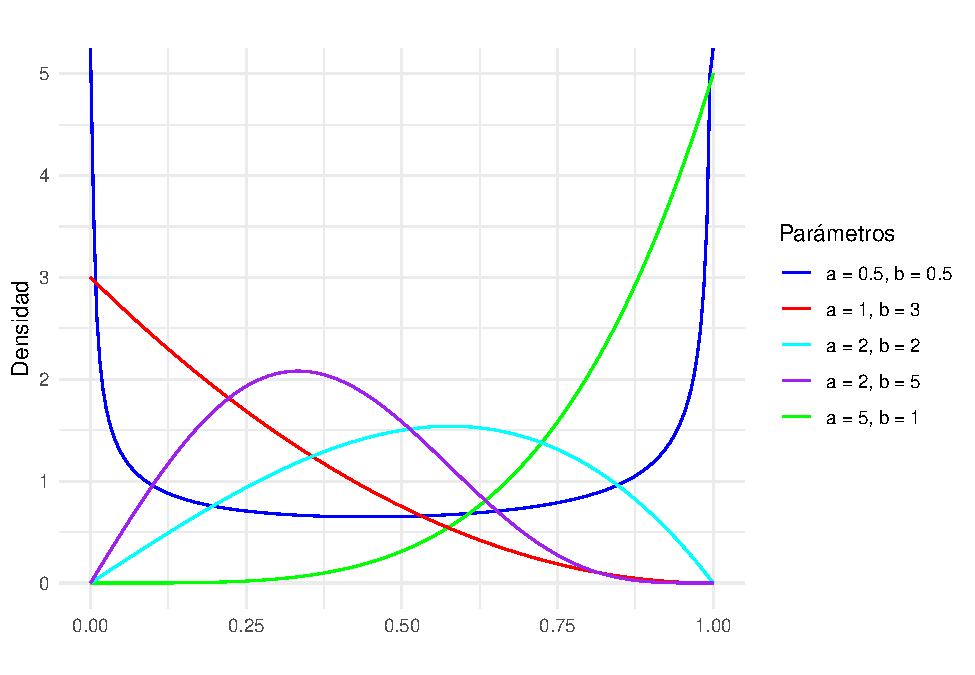
\includegraphics{informe2md_files/figure-latex/unnamed-chunk-5-1} \end{center}

La distribución de Kumaraswamy resulta muy útil a la hora de realizar
estudios bayesianos, ya que presenta una gran flexibilidad y puede
modelar una amplia gama de formas de distribuciones de probabilidad.
Ademas presenta una función de densidad de probabilidad simple y
computacionalmente eficiente, lo que facilita su uso en cálculos
bayesianos. Por último, vale destacar que la restricción al intervalo
\((0;1)\) resulta útil porque se adapta naturalmente al modelado de
proporciones y probabilidades.

\hypertarget{m-h-para-jagdish}{%
\subsection{M-H para Jagdish}\label{m-h-para-jagdish}}

Se utiliza la función construida al comienzo del informe para obtener
5000 muestras de una distribución de Kumaraswamy con parámetros
\(a=6 , b=2\) y una distribución de propuesta beta.

\begin{Shaded}
\begin{Highlighting}[]
\NormalTok{get\_beta\_pars }\OtherTok{\textless{}{-}} \ControlFlowTok{function}\NormalTok{(mu, kappa)\{}
\NormalTok{  alpha }\OtherTok{\textless{}{-}}\NormalTok{ mu }\SpecialCharTok{*}\NormalTok{kappa}
\NormalTok{  beta }\OtherTok{\textless{}{-}}\NormalTok{ (}\DecValTok{1}\SpecialCharTok{{-}}\NormalTok{mu)}\SpecialCharTok{*}\NormalTok{kappa}
  \FunctionTok{return}\NormalTok{(}\FunctionTok{list}\NormalTok{(}\AttributeTok{alpha =}\NormalTok{ alpha, }\AttributeTok{beta =}\NormalTok{ beta))}
\NormalTok{\}}

\NormalTok{d\_objetivo }\OtherTok{\textless{}{-}} \ControlFlowTok{function}\NormalTok{(x, }\AttributeTok{a=}\DecValTok{6}\NormalTok{ ,}\AttributeTok{b=}\DecValTok{2}\NormalTok{)\{}
  \ControlFlowTok{if}\NormalTok{(x}\SpecialCharTok{\textless{}}\DecValTok{0} \SpecialCharTok{||}\NormalTok{ x}\SpecialCharTok{\textgreater{}}\DecValTok{1}\NormalTok{)\{}
\NormalTok{    f}\OtherTok{=}\DecValTok{0}
\NormalTok{  \}}\ControlFlowTok{else}\NormalTok{\{}
\NormalTok{    f }\OtherTok{\textless{}{-}}\NormalTok{ a}\SpecialCharTok{*}\NormalTok{b}\SpecialCharTok{*}\NormalTok{(x}\SpecialCharTok{\^{}}\NormalTok{(a}\DecValTok{{-}1}\NormalTok{))}\SpecialCharTok{*}\NormalTok{(}\DecValTok{1}\SpecialCharTok{{-}}\NormalTok{x}\SpecialCharTok{\^{}}\NormalTok{a)}\SpecialCharTok{\^{}}\NormalTok{(b}\DecValTok{{-}1}\NormalTok{)}
\NormalTok{  \}}
  \FunctionTok{return}\NormalTok{(f)}
\NormalTok{\}}
\end{Highlighting}
\end{Shaded}

Se observan las cadenas obtenidas utilizando tres grados de
concentración distintos \(kappas = 1\), \(25\) y \(50\)

\begin{center}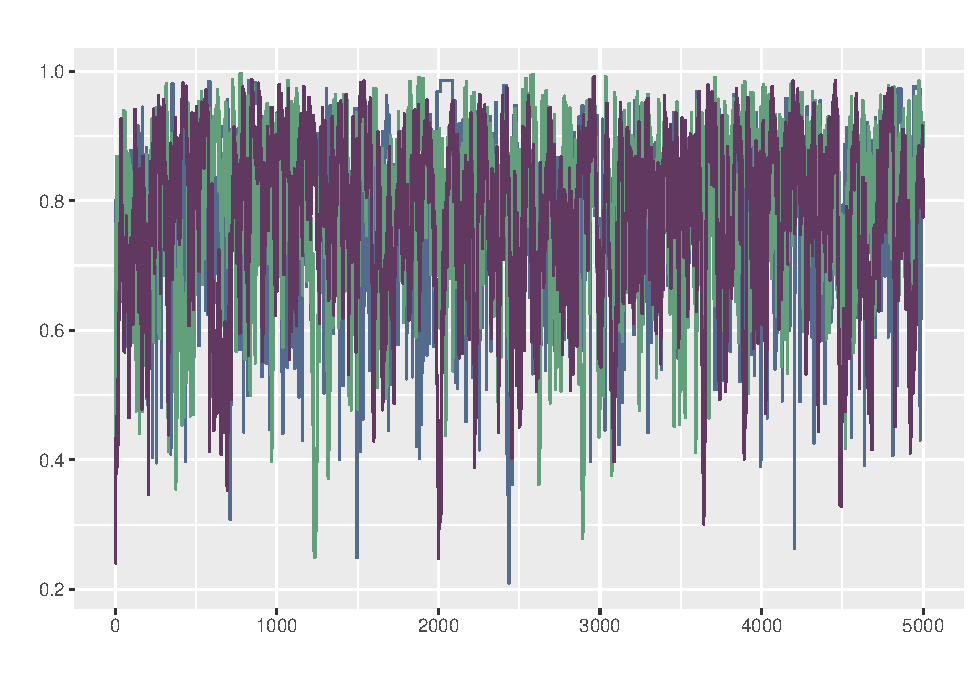
\includegraphics{informe2md_files/figure-latex/unnamed-chunk-7-1} \end{center}

\begin{center}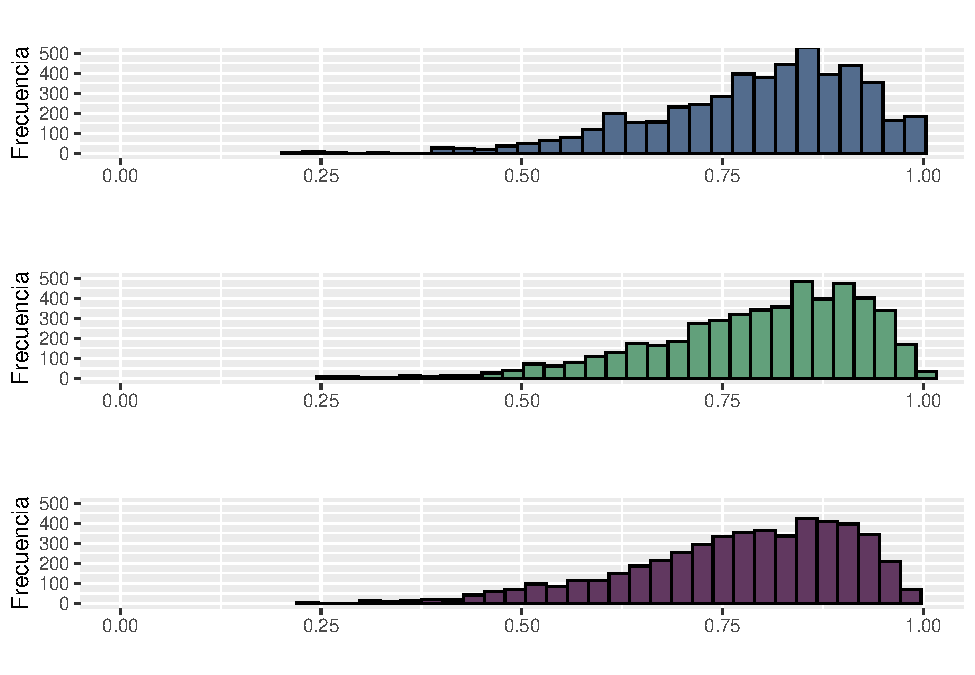
\includegraphics{informe2md_files/figure-latex/unnamed-chunk-8-1} \end{center}

Lo primero que se puede mencionar es la diferencia en las tasas de
aceptación, las cuales fueron \(21.72\) \%, \(77.9\)\% y \(81.66\)\% y
los números efectivos de muestras \(522.36\), \(345.08\) y \(133.14\)
respectivamente. En cuanto a los recorridos de las muestras, se observa
aleatoridad o un patrón de \emph{ruido blanco}. Finalmente observamos el
\(\hat{R}\) el cual resultó ser \(1.003404\) lo que indica converngencia
entren cadenas. Tambien, se presentan histogramas de frecuencias
observadas para las distintas muestras y se observan comportamientos
similares para las tres concentraciones elegidas.

\hypertarget{explorando-cadenas}{%
\subsection{Explorando cadenas}\label{explorando-cadenas}}

Se presenta una tabla con la media de la distribución y los percentiles
5 y 95 de cada una de las cadenas obtenidas.

\begin{longtable}[t]{lrrr}
\toprule
\cellcolor[HTML]{8b7991}{\textcolor{black}{\textbf{}}} & \cellcolor[HTML]{8b7991}{\textcolor{black}{\textbf{Medias}}} & \cellcolor[HTML]{8b7991}{\textcolor{black}{\textbf{Percentil 5}}} & \cellcolor[HTML]{8b7991}{\textcolor{black}{\textbf{Percentil 95}}}\\
\midrule
Kappa = 1 & 0.793 & 0.553 & 0.969\\
Kappa = 25 & 0.800 & 0.550 & 0.963\\
Kappa = 50 & 0.771 & 0.506 & 0.948\\
\bottomrule
\end{longtable}
\newpage

Se replica la misma tabla para el \(logit(x)\) de las muestras.

\begin{longtable}[t]{lrrr}
\toprule
\cellcolor[HTML]{8b7991}{\textcolor{black}{\textbf{}}} & \cellcolor[HTML]{8b7991}{\textcolor{black}{\textbf{Medias}}} & \cellcolor[HTML]{8b7991}{\textcolor{black}{\textbf{Percentil 5}}} & \cellcolor[HTML]{8b7991}{\textcolor{black}{\textbf{Percentil 95}}}\\
\midrule
Kappa = 1 & 1.567 & 0.213 & 3.435\\
Kappa = 25 & 1.624 & 0.202 & 3.267\\
Kappa = 50 & 1.400 & 0.025 & 2.911\\
\bottomrule
\end{longtable}
\newpage

\hypertarget{metropolis-hastings-en-2d}{%
\section{Metropolis-Hastings en 2D}\label{metropolis-hastings-en-2d}}

Para extender el algoritmo de Metropolis-Hastings se generaliza la
función permitiendole implementar el proceso para más de una dimensión.
Se plantea una probabilidad de salto normal bivariada de matriz de
covarianza variable y se otorga flexibilidad al algoritmo haciendo que
reciba como argumento la matriz de covarianza de la probabilidad de
transición.

\begin{Shaded}
\begin{Highlighting}[]
\NormalTok{sample\_mh\_2d }\OtherTok{\textless{}{-}} \ControlFlowTok{function}\NormalTok{ (d\_objetivo, r\_propuesta, d\_propuesta, p\_inicial, n, sigma\_prop)\{}
  \FunctionTok{stopifnot}\NormalTok{(n}\SpecialCharTok{\textgreater{}}\DecValTok{0}\NormalTok{)}
\NormalTok{  salto }\OtherTok{=} \DecValTok{0}
\NormalTok{  muestras }\OtherTok{\textless{}{-}} \FunctionTok{matrix}\NormalTok{(}\AttributeTok{nrow =}\NormalTok{ n, }\AttributeTok{ncol =} \FunctionTok{length}\NormalTok{(p\_inicial))}
\NormalTok{  muestras[}\DecValTok{1}\NormalTok{,]}\OtherTok{\textless{}{-}}\NormalTok{p\_inicial}
  \ControlFlowTok{for}\NormalTok{ (i }\ControlFlowTok{in} \DecValTok{2}\SpecialCharTok{:}\NormalTok{n) \{}
\NormalTok{    p\_actual }\OtherTok{\textless{}{-}}\NormalTok{ muestras[i}\DecValTok{{-}1}\NormalTok{,]}
\NormalTok{    p\_nuevo }\OtherTok{\textless{}{-}} \FunctionTok{r\_propuesta}\NormalTok{(p\_actual)}
\NormalTok{    f\_actual }\OtherTok{\textless{}{-}} \FunctionTok{d\_objetivo}\NormalTok{(p\_actual)}
\NormalTok{    f\_nuevo }\OtherTok{\textless{}{-}} \FunctionTok{d\_objetivo}\NormalTok{(p\_nuevo)}
    
\NormalTok{    q\_actual }\OtherTok{\textless{}{-}} \FunctionTok{d\_propuesta}\NormalTok{(p\_actual,}\AttributeTok{mean=}\NormalTok{p\_nuevo)}
\NormalTok{    q\_nuevo }\OtherTok{\textless{}{-}} \FunctionTok{d\_propuesta}\NormalTok{(p\_nuevo,}\AttributeTok{mean=}\NormalTok{p\_actual)}
    
\NormalTok{    alpha }\OtherTok{\textless{}{-}} \FunctionTok{min}\NormalTok{(}\DecValTok{1}\NormalTok{, (f\_nuevo}\SpecialCharTok{/}\NormalTok{f\_actual)}\SpecialCharTok{*}\NormalTok{(q\_actual}\SpecialCharTok{/}\NormalTok{q\_nuevo))}
    
\NormalTok{    aceptar }\OtherTok{\textless{}{-}} \FunctionTok{rbinom}\NormalTok{(}\DecValTok{1}\NormalTok{,}\DecValTok{1}\NormalTok{, alpha)}
    \ControlFlowTok{if}\NormalTok{ (aceptar)\{}
\NormalTok{      muestras[i,] }\OtherTok{\textless{}{-}}\NormalTok{ p\_nuevo}
\NormalTok{      salto }\OtherTok{=}\NormalTok{ salto }\SpecialCharTok{+} \DecValTok{1}
\NormalTok{    \} }\ControlFlowTok{else}\NormalTok{ \{}
\NormalTok{      muestras[i,] }\OtherTok{\textless{}{-}}\NormalTok{ p\_actual}
\NormalTok{    \}}
    
\NormalTok{  \}}
\NormalTok{  tasa\_acepta }\OtherTok{\textless{}{-}}\NormalTok{ (salto}\SpecialCharTok{/}\NormalTok{n)}\SpecialCharTok{*}\DecValTok{100}
  \CommentTok{\#print(tasa\_acepta)}
  \FunctionTok{return}\NormalTok{ ( muestras ) }
\NormalTok{\}}
\end{Highlighting}
\end{Shaded}

\hypertarget{conociendo-a-mh-en-2d}{%
\subsection{Conociendo a MH en 2D}\label{conociendo-a-mh-en-2d}}

Para comenzar a explorar el comportamiento del algoritmo en dos
dimensiones se obtendrán muestras de una distribución normal bivariada
con media \[ \mu = \begin{pmatrix}
   0.4 \\
   0.75
\end{pmatrix} \] y matriz de covarianza \[\Sigma=\begin{pmatrix}
   0.35 & 0.4 \\
   0.4 & 2.4
\end{pmatrix} \]

Se comienza trazando la densidad de la distribución objetivo para
entenderla mejor y seleccionar un punto inicial que esté dentro de su
rango.

\begin{center}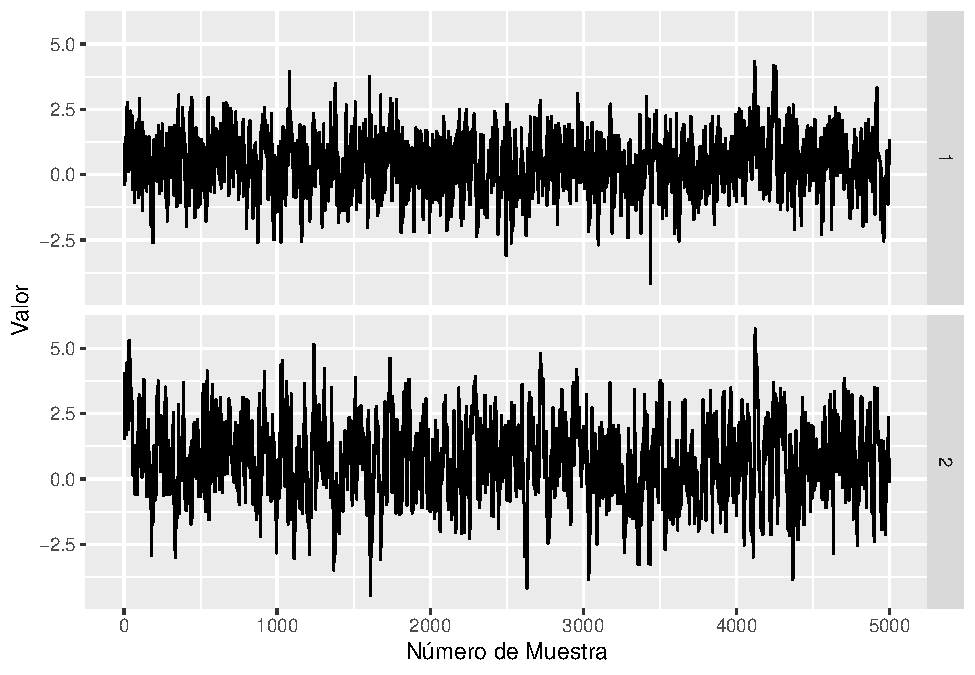
\includegraphics{informe2md_files/figure-latex/unnamed-chunk-17-1} \end{center}

\begin{center}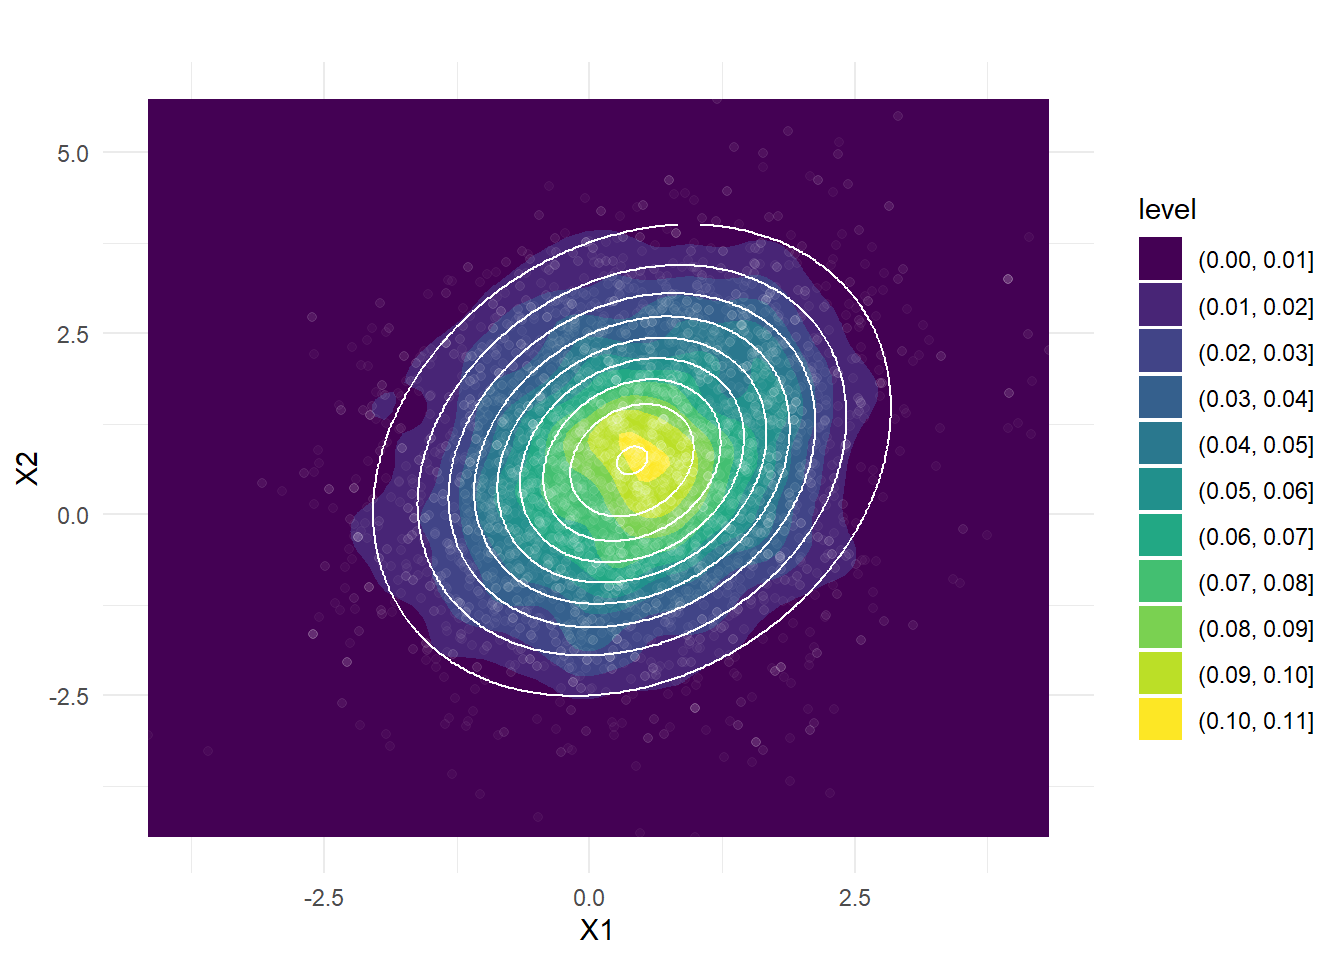
\includegraphics{informe2md_files/figure-latex/unnamed-chunk-18-1} \end{center}

Luego se utiliza la función \textbf{sample\_mh\_2d} para obtener cinco
mil muestras de esta distribución y se grafican.

\begin{center}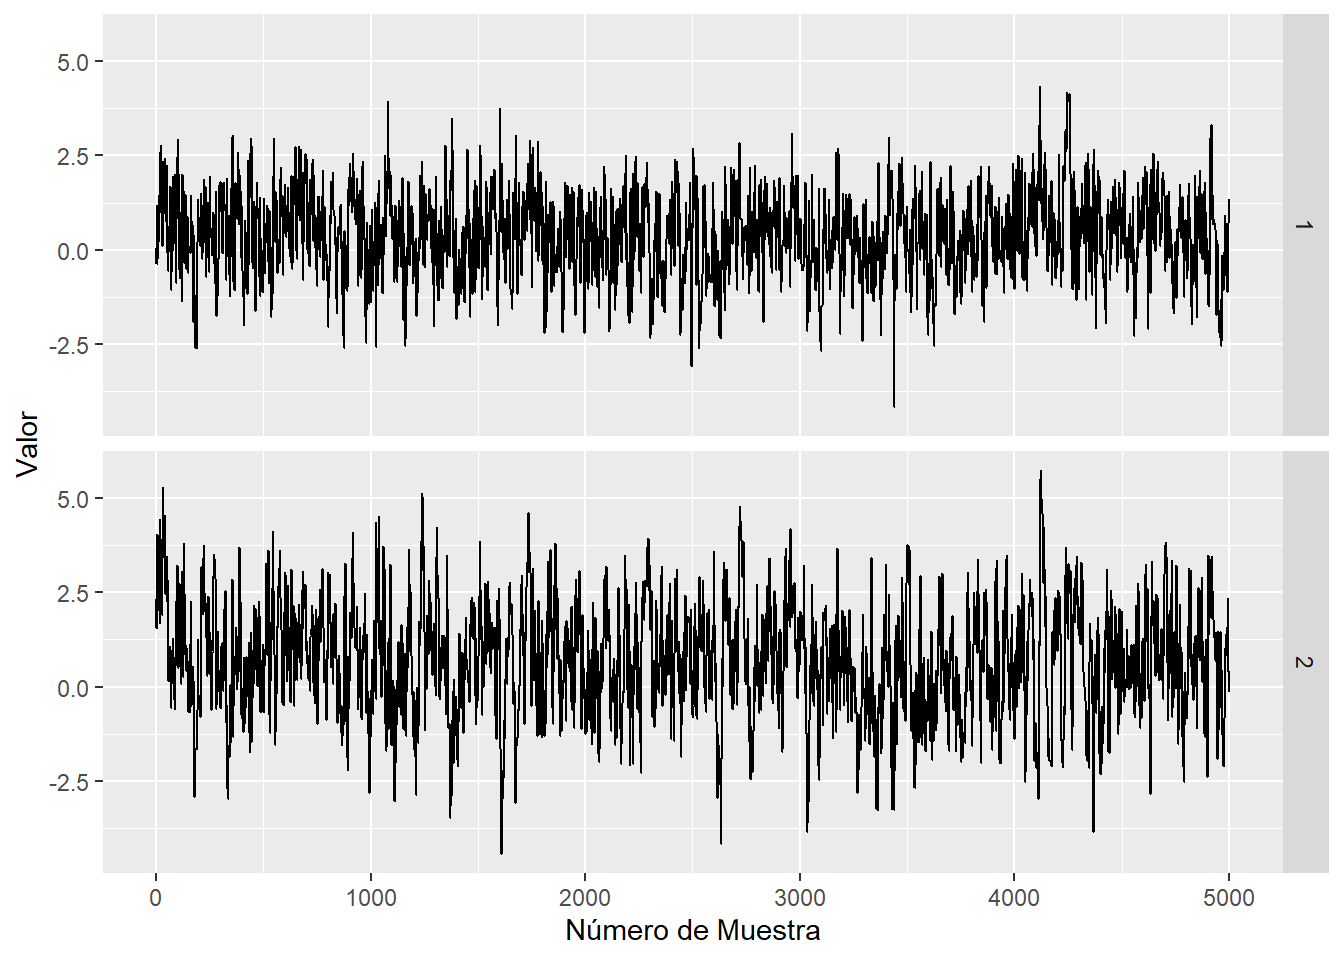
\includegraphics{informe2md_files/figure-latex/unnamed-chunk-19-1} \end{center}

Se presenta a continuación un trace plot para ver la correlación entre
las muestras.

\begin{Shaded}
\begin{Highlighting}[]
\NormalTok{plot\_trace }\OtherTok{\textless{}{-}} \ControlFlowTok{function}\NormalTok{(x, y)\{}
\NormalTok{  n }\OtherTok{\textless{}{-}}\FunctionTok{length}\NormalTok{(x)}
\NormalTok{  df }\OtherTok{\textless{}{-}} \FunctionTok{data.frame}\NormalTok{(}\AttributeTok{x =} \FunctionTok{rep}\NormalTok{(}\DecValTok{1}\SpecialCharTok{:}\NormalTok{n, }\DecValTok{2}\NormalTok{), }\AttributeTok{y =} \FunctionTok{c}\NormalTok{(x, y), }\AttributeTok{dimension =} \FunctionTok{rep}\NormalTok{(}\DecValTok{1}\SpecialCharTok{:}\DecValTok{2}\NormalTok{, }\AttributeTok{each =}\NormalTok{ n))}
  \FunctionTok{ggplot}\NormalTok{(df)}\SpecialCharTok{+}
    \FunctionTok{geom\_line}\NormalTok{(}\FunctionTok{aes}\NormalTok{(}\AttributeTok{x =}\NormalTok{ x, }\AttributeTok{y =}\NormalTok{ y), }\AttributeTok{color =} \StringTok{"\#536C8D"}\NormalTok{)}\SpecialCharTok{+}
    \FunctionTok{facet\_grid}\NormalTok{(}\AttributeTok{rows =} \FunctionTok{vars}\NormalTok{(dimension))}\SpecialCharTok{+}
    \FunctionTok{labs}\NormalTok{(}\AttributeTok{x =} \StringTok{"Muestra"}\NormalTok{, }\AttributeTok{y =} \StringTok{"Valor"}\NormalTok{)}
\NormalTok{\}  }
\FunctionTok{plot\_trace}\NormalTok{(muestras\_2d\_df}\SpecialCharTok{$}\NormalTok{V1, muestras\_2d\_df}\SpecialCharTok{$}\NormalTok{V2)}\SpecialCharTok{+}
  \FunctionTok{theme\_minimal}\NormalTok{()}
\end{Highlighting}
\end{Shaded}

\begin{center}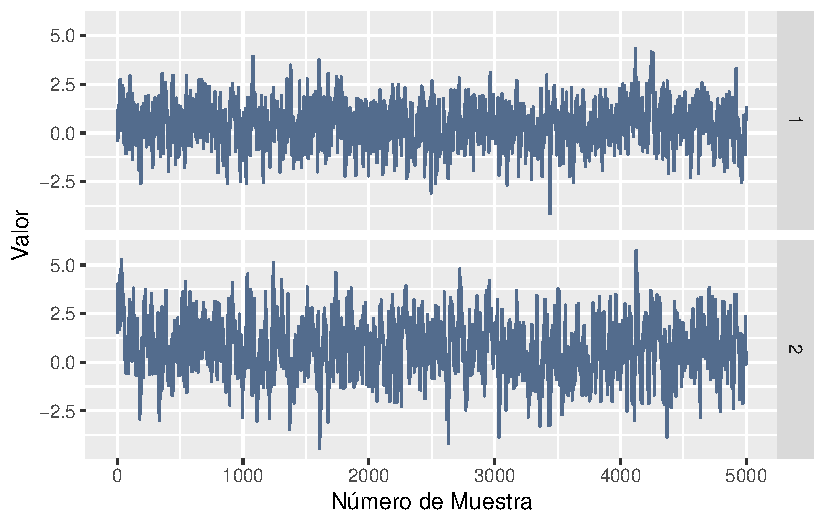
\includegraphics{informe2md_files/figure-latex/unnamed-chunk-20-1} \end{center}

Se observa nuevamente un patrón de \emph{ruido blanco} en los Trace
Plot, lo cual indica una muestra poco correlacionada a través de las
observaciones. Mientras que el número efectivo de muestras para \(X_1\)
es igual a \(481.98\) y para \(X_2\) resulta \(363.31\), lo cual indica
que las cinco mil muestras correlacionadas equivalen a cuatrocientas
ochenta y dos y trecientas secenta y tres muestras independientes,
respectivamente.

A fines de comparar la calidad de las muestras obtenidas, se calculan y
comparan algunas probabilidades mediante distintos métodos.

\begin{longtable}[t]{lrrrr}
\toprule
\cellcolor[HTML]{8b7991}{\textcolor{black}{\textbf{}}} & \cellcolor[HTML]{8b7991}{\textcolor{black}{\textbf{Muestras}}} & \cellcolor[HTML]{8b7991}{\textcolor{black}{\textbf{Montecarlo}}} & \cellcolor[HTML]{8b7991}{\textcolor{black}{\textbf{Grilla}}} & \cellcolor[HTML]{8b7991}{\textcolor{black}{\textbf{Prob. Exacta}}}\\
\midrule
P(X 1> 1, X2 < 0) & 0.0748 & 0.0736 & 0.0691 & 0.0683\\
P(X1 > 1, X2 > 2) & 0.0814 & 0.0850 & 0.0762 & 0.0870\\
P(X1 > 0.4, X2 > 0.75) & 0.2734 & 0.2816 & 0.2775 & 0.2857\\
\bottomrule
\end{longtable}

Como se observa en la tabla, si bien las probabilidades obtenidas
mediante el metodo de Monte Carlo son las que más se aproximan a las
reales, con el método de Metropolis Hasting se obtienen muy buenas
aproximaciones. Vale aclarar que en situaciones más complejas, donde se
dificulta el cálculo de las probabilidades exactas, la aplicación de MH
toma mayor importancia.

\newpage

\hypertarget{funciuxf3n-de-rosenbrock}{%
\section{Función de Rosenbrock}\label{funciuxf3n-de-rosenbrock}}

La función de Rosenbrock, comunmente conocida como la ``banana de
Rosenbrock'', es una función matemática utilizada frecuentemente como un
problema de optimización y prueba para algoritmos de optimización
numérica. También es muy conocida en el campo de la estadística
bayesiana, ya que en ciertos escenarios, la densidad del posterior toma
una forma que definitivamente se asemeja a la banana de Howard
Rosenbrock.

Un ejemplo de esta se presenta a continuación:
\[p^*(x_1, x_2 \mid a, b) = \exp \left\{-\left[(a - x_1) ^ 2 + b(x_2 - x_1^2) ^ 2\right] \right\}\]

\hypertarget{conociendo-a-howard-rosenbrock}{%
\subsection{Conociendo a Howard
Rosenbrock}\label{conociendo-a-howard-rosenbrock}}

El objetivo en este tramo del trabajo es obtener muestras de dicha
función utilizando el algoritmo de Metropolis Hasting, para esto, se
comienza graficandola para conocer su recorrido y asi poder seleccionar
un punto inicial.

\begin{center}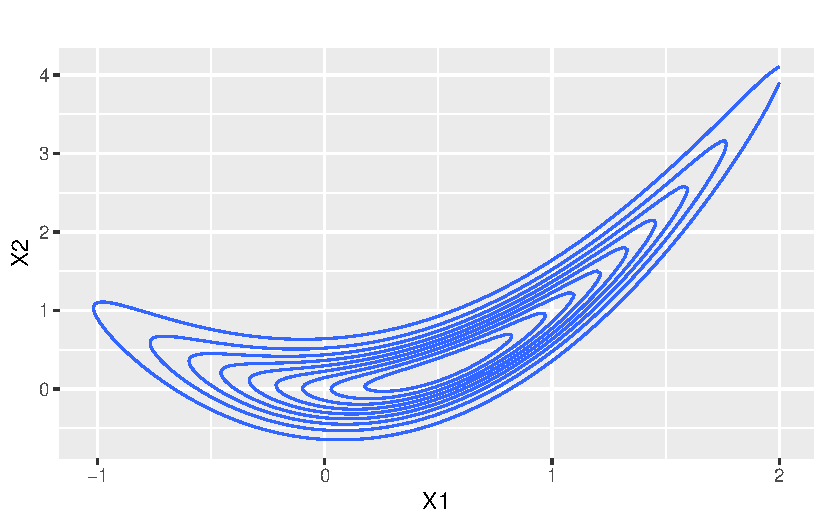
\includegraphics{informe2md_files/figure-latex/unnamed-chunk-25-1} \end{center}

\begin{center}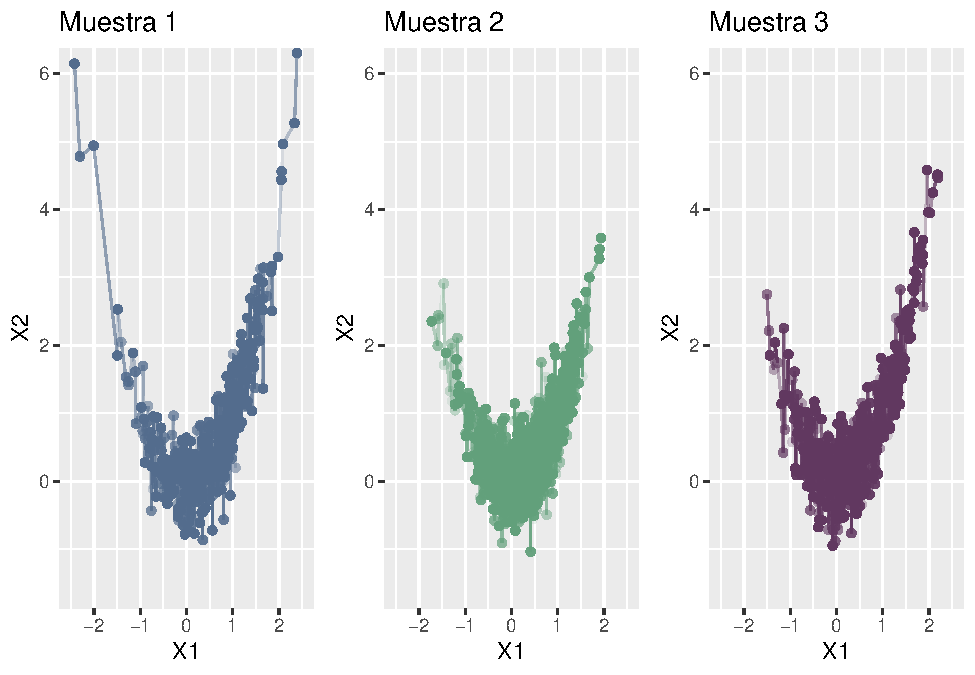
\includegraphics{informe2md_files/figure-latex/unnamed-chunk-26-1} \end{center}

Se obtienen muestras utilizando tres matrices de covariancias distintas
para la distribución que propone los saltos. Estas son:
\[\Sigma_1=\begin{pmatrix}
   4 & 1 \\
   1 & 4
\end{pmatrix} \] Las muestras del primer \emph{posterior} resultan de la
forma

\begin{center}\includegraphics{informe2md_files/figure-latex/unnamed-chunk-28-1} \end{center}

\[\Sigma_2=\begin{pmatrix}
   1 & 0 \\
   0 & 1
\end{pmatrix} \] Las muestrar del segundo \emph{posterior} obtenida
resultan de la forma

\begin{center}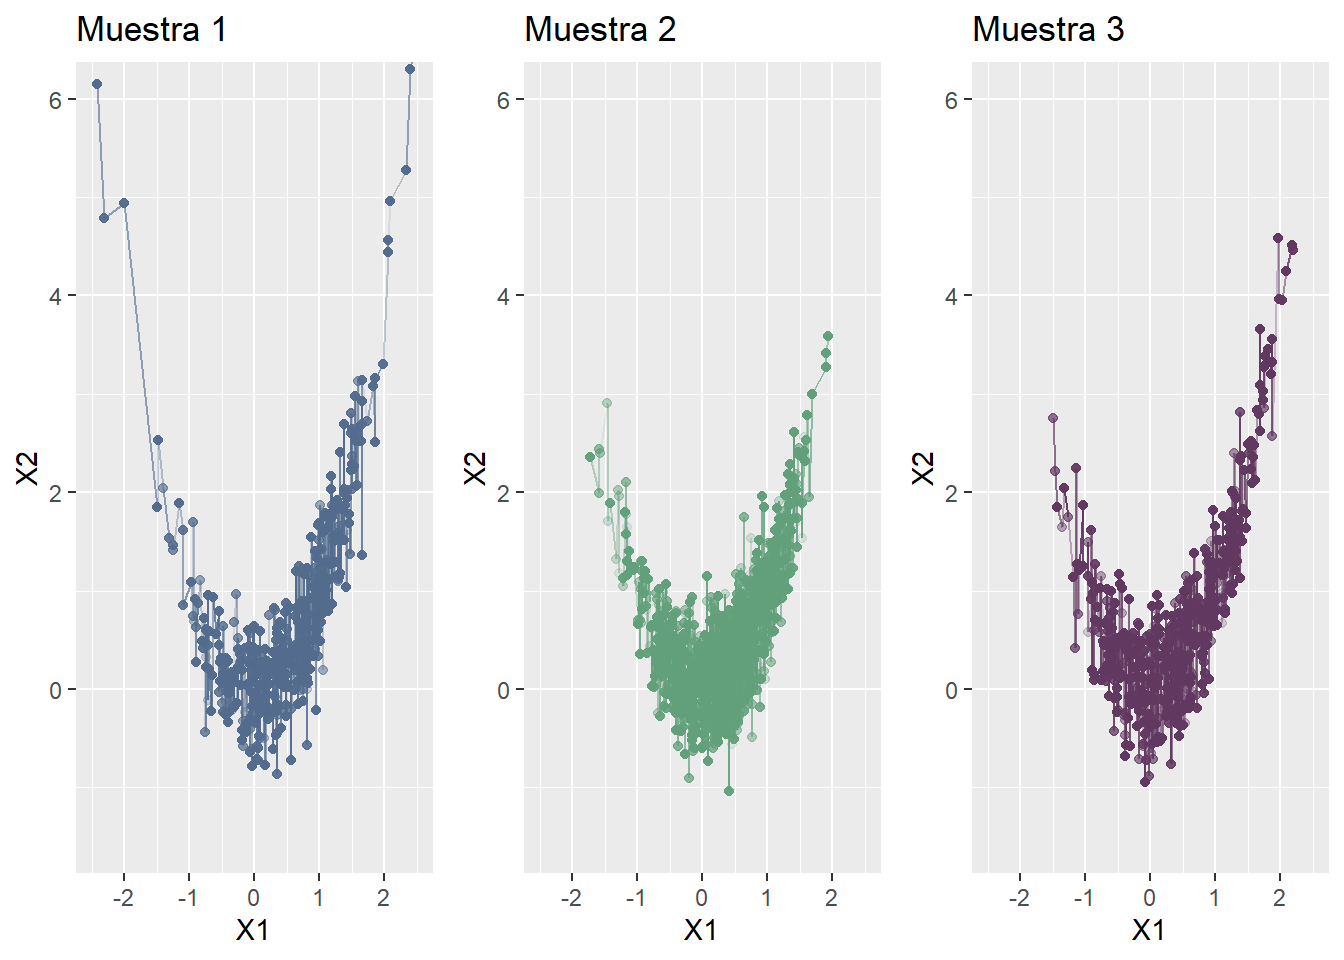
\includegraphics{informe2md_files/figure-latex/unnamed-chunk-29-1} \end{center}

\[\Sigma_3=\begin{pmatrix}
   2 & -2 \\
   -2 & 5
\end{pmatrix} \] Las muestrar del tercer \emph{posterior} obtenida
resultan de la forma

\begin{center}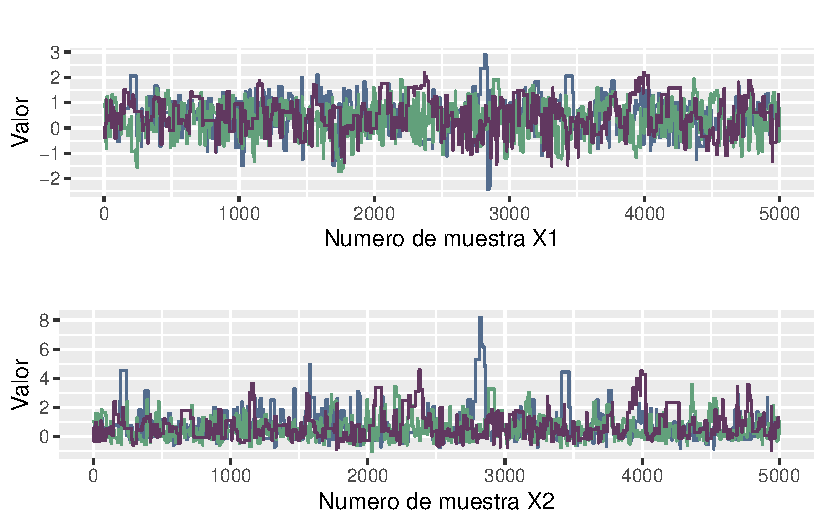
\includegraphics{informe2md_files/figure-latex/unnamed-chunk-30-1} \end{center}

Se comparan las trayectorias para las distintas muestras obtenidas, y
posteriormente se analizan las funciones de autocorrelación:

\begin{center}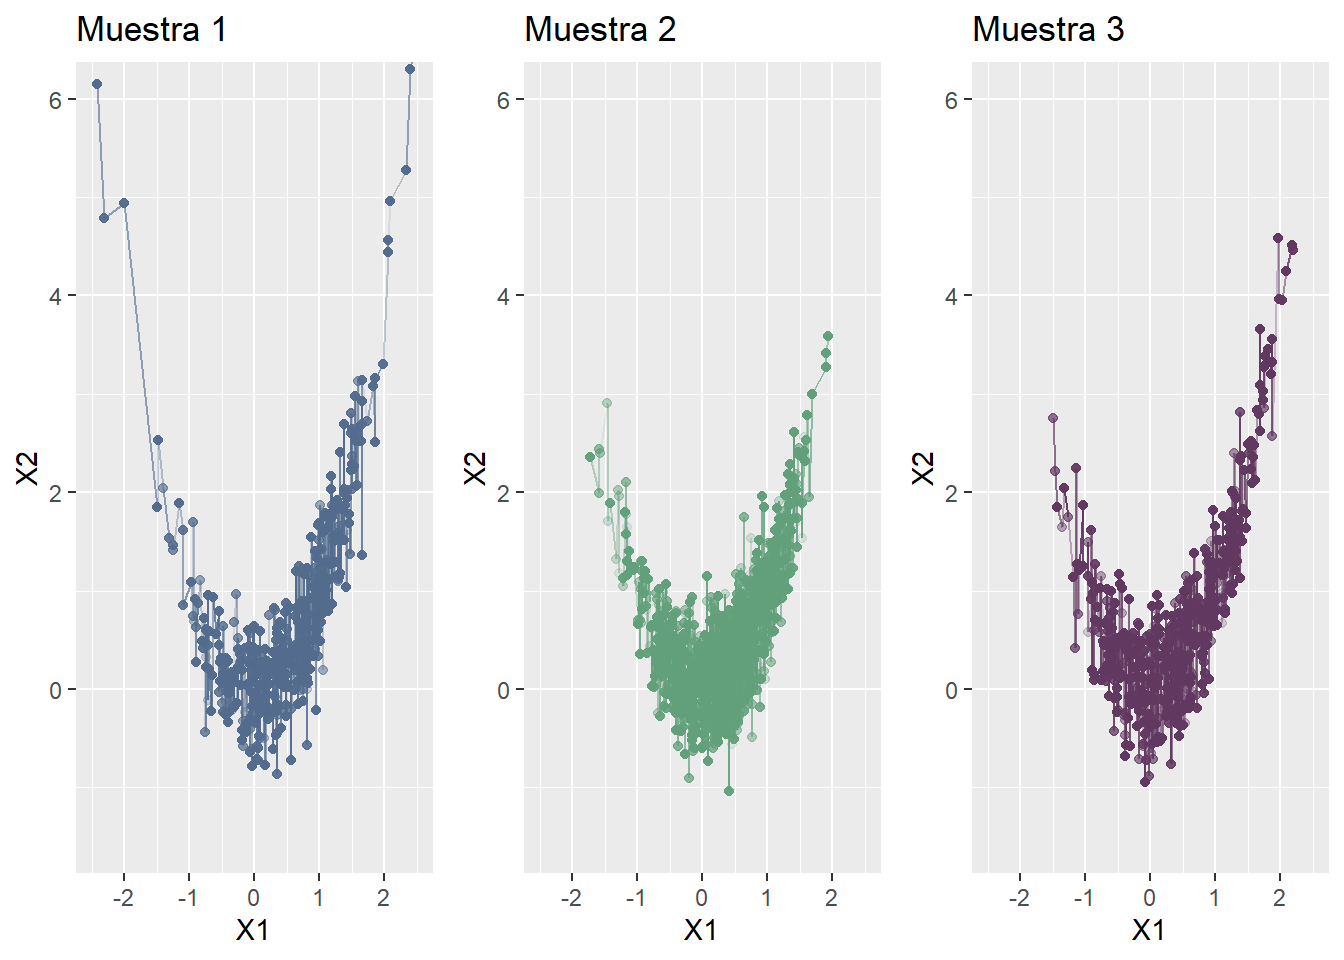
\includegraphics[width=1\linewidth]{informe2md_files/figure-latex/unnamed-chunk-31-1} \end{center}

Se observa que la trayectoria de la primera y tercera muestra parecen
presentar valores en todo el recorrido de la función de Rosenbrock,
mientras que la muestra obtenida con la segunda cadena se restringe a
los valores centrales de dicha función.

A continuación se presentan los \emph{trace plot}, gráficos de
autocorrelación y números efectivos de muestras a fin de comparar cómo
se comporta el método según la matriz de covariancia propuesta que se
utilice.

\begin{center}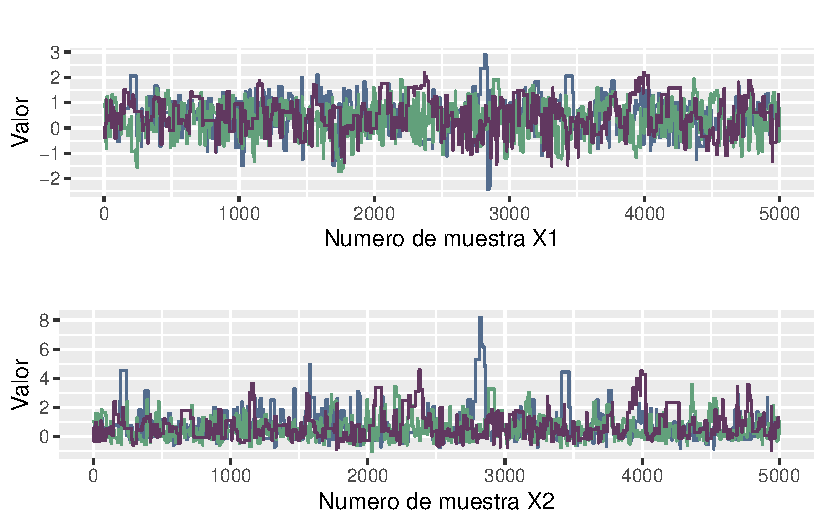
\includegraphics{informe2md_files/figure-latex/unnamed-chunk-32-1} \end{center}

\begin{center}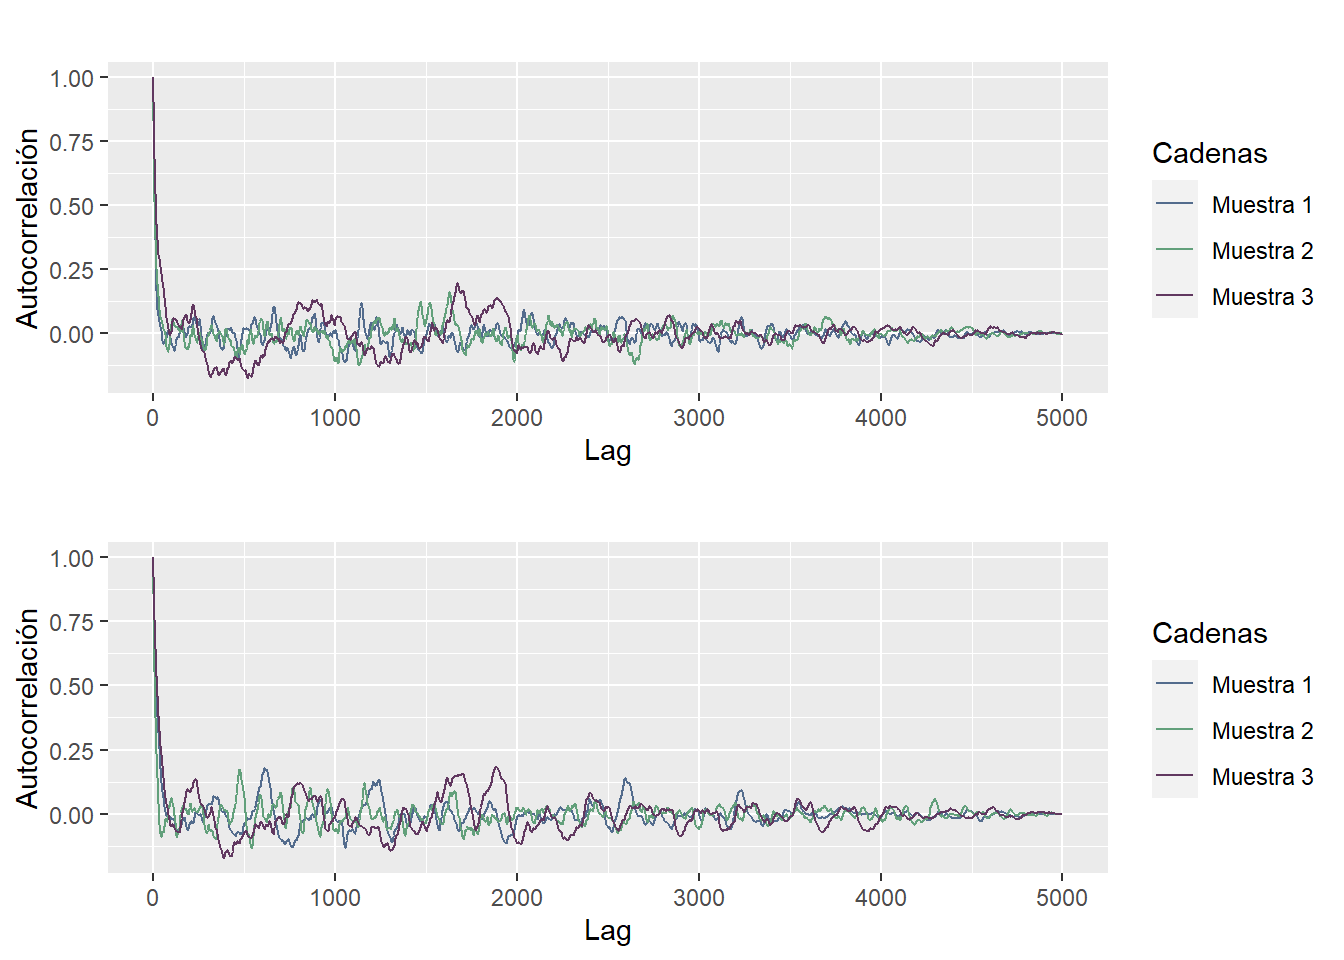
\includegraphics{informe2md_files/figure-latex/unnamed-chunk-32-2} \end{center}

\begin{longtable}[t]{lrr}
\toprule
\cellcolor[HTML]{8b7991}{\textcolor{black}{\textbf{}}} & \cellcolor[HTML]{8b7991}{\textcolor{black}{\textbf{N° efectivo de muestras para X1}}} & \cellcolor[HTML]{8b7991}{\textcolor{black}{\textbf{N° efectivo de muestras para X2}}}\\
\midrule
Muestra 1 & 218.43 & 113.38\\
Muestra 2 & 185.14 & 214.42\\
Muestra 3 & 98.23 & 92.24\\
\bottomrule
\end{longtable}

A diferencia de las muestras 1 y 2, la tercera muestra presenta una
mayor autocorrelación en sus observaciones, y debido a esto se puede
observar que también el número efectivo de muestras disminuye
prácticamente en la mitad de las observaciones. Además la probabilidad
de aceptación para la primer cadena es \(8.24\), es decir que el
algoritmo acepta el \(8.24\)\% de los pasos propuestos, significando que
queda muchas veces con el mismo valor de la muestra. Similar ocurre con
la cadena 3 que acepta el \(10.28\) de las veces, mientras que el mayor
porcentaje de aceptación es de la cadena 3 con un \(19.22\)\%. Todas
estas interpretaciones podrían deberse a que las matrices de covarianzas
utilizadas en las cadenas 1 y 3 no acompañan la forma de la distribución
a posteriori y son muy amplias, mientras que en la 2 se concentra más en
los valores centrales de la distribución y sigue más su forma.

Nuevamente, con el motivo de analizar la calidad de las muestras
obtenidas, se calculan y comparan algunas probabilidades utilizando las
muestras, el método de la grilla y el método de Monte Carlo. Dichas
probabilidades se calculan con las muestras de la cadena 2, la cual
presenta el mayor número efectivo de muestras.

\begin{longtable}[t]{lrrrr}
\toprule
\cellcolor[HTML]{8b7991}{\textcolor{black}{\textbf{}}} & \cellcolor[HTML]{8b7991}{\textcolor{black}{\textbf{Muestras}}} & \cellcolor[HTML]{8b7991}{\textcolor{black}{\textbf{Montecarlo}}} & \cellcolor[HTML]{8b7991}{\textcolor{black}{\textbf{Grilla}}} & \cellcolor[HTML]{8b7991}{\textcolor{black}{\textbf{Prob. Exacta}}}\\
\midrule
P(0 < X1 < 1 ; 0 < X2 < 1) & 0.3896 & 0.5164 & 0.3697 & 0.5137\\
P(-1 < X1 < 0 ; 0 < X2 < 1) & 0.1478 & 0.2041 & 0.1444 & 0.2022\\
P(1 < X1 < 2 ; 2 < X2 < 3) & 0.0298 & 0.0872 & 0.0605 & 0.0838\\
\bottomrule
\end{longtable}

Estos resultados exponen una debilidad en el algoritmo de Metropolis
Hasting. Se observan importantes diferencias entre las probabilidades
calculadas con MH o grilla en comparación a las probabilidades
calculadas con Monte Carlo o integración exacta (estos últimos dos
metodos, más precisos).

\hypertarget{conclusiones}{%
\section{Conclusiones}\label{conclusiones}}

A lo largo del trabajo, se observa que Metropolis Hastings es una
variante que permite sacar muestras de distribuciones de probabilidad,
incluso cuando no se tiene idea de cómo es exactamente esa distribución,
sólo se necesita su ley. Se ha probado en distribuciones
unidimensionales y bidimensionales, como las distribuciones de
Kumaraswamy y Rosenbrock. Se ha interactuado con diferentes formas de
distribución propuesta y se ha observado cómo esta afecta a la
eficiencia del algoritmo. Sin embargo, se han identificado algunas
debilidades, por ejemplo, su rendimiento puede ser sensible a la
elección de la distribución propuesta, lo que puede afectar la
eficiencia y la convergencia del algoritmo. Además, puede ser
computacionalmente costoso para dimensiones muy altas o distribuciones
multimodales.

Es interesante ver a Metropolis Hastings como una herramienta en
estadística bayesiana, ya que ayuda a muestrear y/o graficar
distribuciones a posteriori. No obstante, se conocen métodos más
precisos para obtener muestras de distribuciones complejas, como por
ejemplo, Hamiltonian - Monte Carlo.

\end{document}
